% Tea-time talk: Claude-based classification of Socratic math hints
% Build:  tectonic tea_time_talk.tex   (or pdflatex, run twice)
% Figures are read from local copies in outputs_llms/ and outputs/ (Overleaf-ready),
% falling back to ../outputs_llms/ and ../outputs/ -- to regenerate, run the pipeline:
%   uv run socratic-hints all-llm && uv run socratic-hints plot-types-llm
\documentclass[10pt,aspectratio=169]{beamer}

\usetheme{Madrid}
\usecolortheme{seahorse}
\usepackage{graphicx}
\usepackage{booktabs}
\usepackage{amsmath}
% Beamer already loads hyperref; configure it here instead of \usepackage.
% Leaving linkcolor empty keeps beamer's internal links (TOC, navigation)
% in the theme's own colors; only URLs are forced blue.
\hypersetup{colorlinks=true, urlcolor=blue, linkcolor=}
\graphicspath{{outputs_llms/}{outputs/}{../outputs_llms/}{../outputs/}}

\setbeamertemplate{navigation symbols}{}
\newcommand{\good}[1]{\textcolor{blue}{#1}}
\newcommand{\bad}[1]{\textcolor{red}{#1}}
\newcommand{\hf}{\textcolor{blue}{[f]}}
\newcommand{\hr}{\textcolor{teal}{[r]}}
\newcommand{\hb}{\textcolor{orange}{[b]}}
\newcommand{\he}{\textcolor{purple}{[e]}}

\title[From Hints to Textbooks]{From Hints to Textbooks}
\subtitle{Studying Scaffolds through Bayesian Methods and LLMs}
\author{Justin Stevens}
%\institute{Amii Team Time Talks}
\date{\today}

\begin{document}

\begin{frame}
  \titlepage
\end{frame}

\begin{frame}{The problem \& questions }
\begin{itemize}
    \item Many students are using LLMs for education 
    \begin{itemize} 
    \item Last summer, I gave an \href{https://www.youtube.com/watch?v=ECm2GY9uZN8}{AI Seminar on Intelligent Tutoring Systems}
    \item Hints are an important part of Intelligent Tutoring Systems
    \end{itemize} 
    \medskip  
    \item Can we learn about the types of hints LLMs provide learners by automatically classifying the hints?
    \medskip  
    \item Can we learn about the distribution of problem types that can help inform pedagogical decisions?
\end{itemize}
\end{frame}

% ===========================================================================
\section{Dataset and Methodology}
% ===========================================================================

\begin{frame}{The dataset: SocraticMath}
  \begin{columns}[T]
    \column{0.58\textwidth}
    \textbf{Where it comes from}
    \begin{itemize}
      \item Competition problems from the MATH benchmark\footnote{\tiny Hendrycks et al., \emph{Measuring Mathematical Problem Solving with the MATH Dataset}, NeurIPS 2021.}, each augmented with a
            \emph{chain of Socratic questions}\footnote{\tiny Ding et al., \emph{Boosting LLMs with Socratic Method for Conversational Mathematics Teaching}, CIKM 2024.}
      \item One JSON file per problem:
            \texttt{problem}, \texttt{level} (1--5), \texttt{solution}, \texttt{type},
     \texttt{socratic\_questions}
    \end{itemize}
    \medskip
    
    \textbf{Scale}
    \begin{itemize}
      \item 7 domains $\times$ 565--590 problems $=$ \textbf{4{,}043 problems}
      \item \textbf{31{,}613 Socratic hints} ($\approx$ 7.8 per problem)
    \end{itemize}
    \column{0.38\textwidth}
    
    \begin{center}
      \small
      \begin{tabular}{lr}
        \toprule
        domain & problems \\
        \midrule
        algebra & 576 \\
        counting \& probability & 584 \\
        geometry & 575 \\
        intermediate algebra & 565 \\
        number theory & 583 \\
        prealgebra & 590 \\
        precalculus & 570 \\
        \midrule
        total & 4{,}043 \\
        \bottomrule
      \end{tabular}
    \end{center}
  \end{columns}
\end{frame}

\begin{frame}{Taxonomy 1: four hint types}
  Goldin, Koedinger \& Aleven (2013) plus one extra type for Socratic chains:
  \medskip
  \begin{description}
    \item[\hf~feature-pointing] draws attention to a specific aspect of this problem \\ {\small ``Notice that these two angles are vertical angles''}  
    \item[\hr~principle-stating] supplies a general rule, definition, or theorem \\ 
          {\small ``Vertical angles are equal in measure''}  
    \item[\hb~bottom-out] directly advances the solution to set up, substitute, solve, etc. \\
          {\small ``Add these two known angles to find the missing one''}  
    \item[\he~extension] pushes past the current problem to think of applications, generalizations \\
          {\small ``Can you think of other situations where this matters?''}  
  \end{description}
  \medskip
   
    Goal: learn a $4\times4$ \textbf{transition matrix} $M$ per group, where $p_{ij}$ is the probability the next hint is type $j$ given the current one is type $i$.

\end{frame}

\begin{frame}{A worked example (algebra \texttt{hint\_0})}
  \small
  Let
  $f(x)=\begin{cases} ax+3 & x>2\\ x-5 & -2\le x\le 2\\ 2x-b & x<-2 \end{cases}$.
  \quad Find $a+b$ if $f$ is continuous.
  \medskip
  \begin{enumerate}\footnotesize
    \item Can you explain what a piecewise function is and how it is represented algebraically?  ~\hf  
    \item How would you determine if the function is continuous where different pieces meet?  ~\hr  
    \item What conditions need to be satisfied for a piecewise function to be continuous? ~\hf  
    \item Can you identify the value of $a$ and $b$ that would make the function continuous? ~\hb  
    \item How would you approach solving for $a$ and $b$? ~\hb  
    \item Are there any restrictions or constraints on the values of $a$ and $b$? ~\hb  
    \item Can you explain the significance of continuity in real-life applications? ~\he  
    \item Can you think of other examples where continuity is important? ~\he  
  \end{enumerate}
  \medskip
  \normalsize
  Labels shown are my hand labels. On this chain
  \good{Claude validates all 8/8 labels }
\end{frame}


\begin{frame}{Method: one Claude call per problem, two classifications}
  \begin{itemize}
    \item \texttt{claude-opus-4-8} receives the problem, difficulty level, worked solution, and the numbered Socratic chain, and returns strict JSON:
    \begin{enumerate}
      \item one hint label (\texttt{f/r/b/e}) per question, in order
      \item one Quarfoot type for the whole problem
    \end{enumerate}
    \item Prompt contains both taxonomies' definitions + the worked example above as a few-shot prompt 
    \item Every response is \textbf{validated} to make sure it is in the correct output format and retried on failure. 
    \item Downstream analysis: group the chains (by domain, or by problem type), count
          transitions, Dirichlet--multinomial posterior per group, row-averaged
          symmetrized KL, similarity $e^{-KL}$
  \end{itemize}
\end{frame}


% ===========================================================================
\section{Headline 1: Counting \& Probability is different}
% ===========================================================================

\begin{frame}{Counting \& Probability Transition Matrix}
  Per-domain $4\times4$ matrices over \hf\hr\hb\he. Six of the seven look
  roughly like algebra's. One doesn't:
  \begin{align*}
    M_{\text{algebra}}=\begin{pmatrix}
      \mathbf{0.227} & 0.224 & 0.498 & 0.051\\
      0.160 & 0.272 & 0.502 & 0.067\\
      0.089 & 0.158 & 0.600 & 0.153\\
      0.030 & 0.073 & \mathbf{0.193} & \mathbf{0.704}
    \end{pmatrix}
    \quad
    M_{\text{count.\ \& prob.}}=\begin{pmatrix}
      \mathbf{0.418} & 0.126 & 0.421 & 0.035\\
      0.184 & 0.242 & 0.441 & 0.133\\
      0.070 & 0.104 & 0.715 & 0.111\\
      0.030 & 0.060 & \mathbf{0.079} & \mathbf{0.831}
    \end{pmatrix}
  \end{align*}
  \begin{itemize}
    \item $f\!\to\!f = 0.418$: the highest of \emph{any} domain and nearly \textbf{2$\times$} algebra's 0.227 
    \item $e\!\to\!b = 0.079$: the lowest of any domain and $e\!\to\!e = 0.831$
  \end{itemize}
\end{frame}



\begin{frame}{Across all 21 pairs: Counting \& Probability is the outlier}
    \begin{center}
      
\includegraphics[height=0.80\textheight]{similarity_symmetric.png}
    \end{center}
\end{frame}

\begin{frame}{Marginal Hint Distribution}
  \begin{itemize}
    \item Its hint \emph{marginals} stand out as the most feature-pointing, least principle-stating of any domain: 
      \begin{center}
        \small
        \begin{tabular}{lcccc}
          \toprule
          & f & r & b & e \\
          \midrule
          counting \& probability & \textbf{23.9\%} & \textbf{13.9\%} & 50.0\% & 12.1\% \\
          all domains (pooled)    & 19.0\% & 18.6\% & 51.5\% & 10.9\% \\
          \bottomrule
        \end{tabular}
      \end{center}
       
      \medskip 
    \item Intuition: ``notice how many ways\ldots'' (a feature pointing hint ~\hf) is more common in counting \& probability than ``recall the theorem\ldots'' (a principle-stating hint ~\hr)
  \end{itemize}
\end{frame}

% ===========================================================================
\section{Headline 2: Complex Problems contain more Bottom Out Hints}
% ===========================================================================
% Numbers in this section are computed from the pipeline's
% outputs_llms/classified_hints.csv and problem_type_analysis_summary.json:
% per-problem transition counts aggregated over FN/AC/CH/ET vs IM/IN/FP/SP/MP,
% all-ones Dirichlet prior, row-averaged symmetrized KL (0.0386), and a
% problem-level permutation test (10,000 shuffles of the half assignment, seed 0).

\begin{frame}{Taxonomy 2: Quarfoot's nine problem types}
  A musical metaphor, ordered (roughly) least $\to$ most mathematical substance: \footnote{The Music of Mathematics: Toward a New Problem Typology, \textit{David Quarfoot PhD thesis}, UCSD}  
  \medskip
  \begin{center}
    \small
    \begin{tabular}{llp{0.6\textwidth}}
      \toprule
      & type & what it is \\
      \midrule
      FN & First Notes & one-step, single-path, algorithmic; fluency \\  
      AC & Accidentals & looks routine, hides a twist; targets a misconception \\  
      CH & Chords & one idea, several steps; deepens a single concept \\  
      ET & Etudes & drills one technique; word-problem dressing \\  
      IM & Improvisations & a playground; first attempts fail, so you experiment \\  
      IN & Interpretations & wide-open solution space; compare qualitatively different paths \\  
      FP & First Pieces & first problems needing multiple ideas plus a macro-level plan \\  
      SP & Showpieces & very hard, hinges on a flash of insight; cognitive \\  
      MP & Masterpieces & many skills converging on a generalizable truth; capstones \\
      \bottomrule
    \end{tabular}
  \end{center}
\end{frame}

\begin{frame}{Comparing Routine vs. Complex Problem Types}
  Group the hints by classification of \emph{Quarfoot type}, split into \textbf{routine} vs. \textbf{complex}  

  \bigskip 

  The mean level of the problems in the \textbf{routine} group is 2.86/5, and in the \textbf{complex} group is 4.51/5

  \bigskip  
  Similarity $e^{-0.0386} = \mathbf{0.962}$; only \textbf{4 of 21} domain pairs
  are farther apart (all with counting \& probability)
\end{frame}


\begin{frame}{Breakdown of Routine vs. Complex Problems}
  \begin{table} 
    \centering 
    \small
    \begin{tabular}{lrccc}
      \toprule
      type & $n$ & Principle Stating Marginal & $b\to b$ & Extension Marginal \\
      \midrule
      First Notes & 658   & 26\% & 0.56 & 18\% \\
      Accidentals & 289   & 20\% & 0.63 & 12\%  \\
      Chords & 1{,}501 & 21\% & 0.63 & 12\%  \\
      Etudes & 432   & 14\% & 0.69 & 11\%  \\
      \midrule
      Improvisations & 13    & 14\% & 0.64 & 13\%  \\
      First Pieces & 661   & 14\% & 0.77 & 6\%  \\
      Showpieces & 487   & 12\% & 0.78 & 6\%  \\
      Masterpieces & 2     & --- & ---  & ---  \\
      \bottomrule
    \end{tabular}
    
    \vspace{0.75em} % Adds breathing room between table and text
    
    \begin{minipage}{0.95\textwidth}
      \footnotesize % Drops font size slightly below the table's \small  
      \textbf{Routine problems:} Often principle-stating; hints state the principle~\hr, then generalize away the problem~\he. 
      
      \vspace{0.3em}
        
      \textbf{Complex problems:} No single rule solves them all, so hints enumerate the plan instead (higher $\hb\to\hb$). 
    \end{minipage}
  \end{table} 
\end{frame}


\begin{frame}{First Pieces (Complex) Counting \& Probability Problem }
  \textbf{Problem:} Four standard six-sided dice are rolled. If the product of their values is even, what
  is the probability their sum is odd? 
  \smallskip
  \begin{enumerate}
    \item[1.] \hf~Can you explain the problem statement in your own words?
    \item[2.] \hr~What is the condition for the product of the dice values to be even?
    \item[3.] \hb~If all the dice rolls yield odd numbers, how many possible outcomes are there?
    \item[4.] \hb~How many possible outcomes are there in total?
    \item[5.] \hb~How can we determine the number of outcomes where at least one even number is rolled?
    \item[] \hspace{1.2em}$\vdots$\hspace{0.8em} {\footnotesize seven more \hb: split into
            cases by how many dice are odd, count each case, combine}
    \item[13.] \hb~What is the desired probability of the sum being odd?
    \item[14.] \hb~Can you simplify the fraction to its lowest terms?
    \item[15.] \hb~What is your final answer for the probability?
  \end{enumerate}
\end{frame}


% ===========================================================================
\section{My Olympiad Number Theory Book vs.\ MATH number theory}
% ===========================================================================

\begin{frame}{Olympiad Number Theory by Justin Stevens}

INSERT QR CODE HERE 

\end{frame}

\begin{frame}{The nine types with problems from my Olympiad Number Theory book}
  \begin{center}
    \small
    \begin{tabular}{lp{0.66\textwidth}l}
      \toprule
      type & problem & source \\
      \midrule
      First Notes & Find $x$ such that $1+x+x^2+x^3+\cdots=4$. & Mandelbrot \\
      Accidentals & Show there are no integers $x,y$ with $1691x+1349y=1$. & Ch.\ 5 \\
      Chords & The sum of 18 consecutive positive integers is a perfect square. Find the smallest possible such sum. & AMC 12 \\
      Etudes & Compute $\displaystyle \sum_{m=1}^{75}(2+3m)$. & Ch.\ 1 \\
      Improvisations & Pages numbered $1$--$n$; one page number was accidentally added twice, giving $1986$. Which page? & AIME \\
      Interpretations & Prove these Fibonacci identities \emph{in two different ways}. & Ch.\ 2 \\
      First Pieces & Find the 8th term of $1440, 1716, 1848,\ldots$, formed by multiplying corresponding terms of two arithmetic sequences. & AIME \\
      Showpieces & Evaluate $\displaystyle \prod_{n=2}^{\infty}\frac{n^3-1}{n^3+1}$. & Putnam \\
      Masterpieces & Prove every positive integer is a sum of non-consecutive Fibonacci numbers. & Zeckendorf \\
      \bottomrule
    \end{tabular}
  \end{center}
\end{frame}

\begin{frame}{Problem Distribution: My Book vs. Number Theory MATH datset}
  \begin{center}
    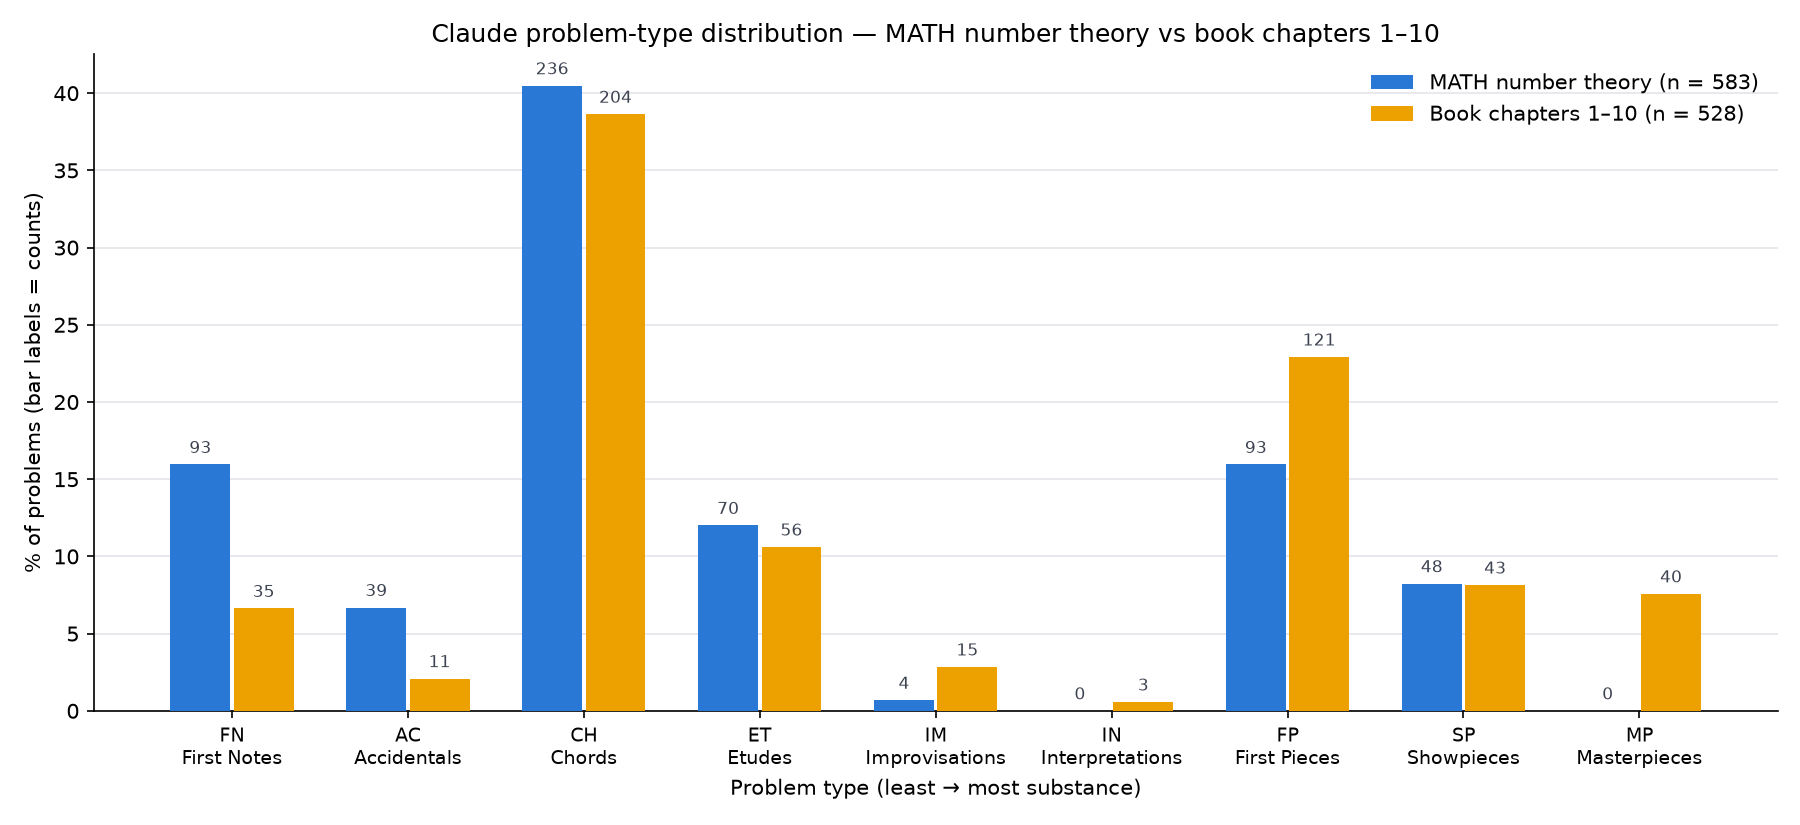
\includegraphics[height=0.77\textheight]{problem_type_hist_number_theory_vs_book.png}
  \end{center}
\end{frame}



\begin{frame}{What this offers textbook authors}
  \begin{itemize}
    \item \textbf{An audit tool for the selection of your problem}: See if it matches the desired distribution.
    \bigskip 
    \item \textbf{A check on the pedagogical arc}: Do problems get more complex in later chapters? 
    \bigskip 
    \item \textbf{Gap-finding}: Discovered there are virtually no interpretation questions in my book. 
    \end{itemize} 
\end{frame}

\begin{frame}{Future Steps \& Limitations}
\begin{enumerate} 
\item Create a human-labeled evaluation set \bigskip 
\item Have Claude solve the problems itself instead of seeing worked solutions \bigskip 
\item Compute Cohen's $\kappa$ of inter-rater reliability coefficient with a second LLM  annotator
\end{enumerate}

\end{frame} 

\begin{frame}{AI Disclaimer}
Claude's Anthropic Opus 4.8 \& Fable models were used to assist with writing code and analysis and to help create a first draft of these slides, which were then refined by me to deliver this presentation. 

\end{frame}


\begin{frame}{Recap}

\tableofcontents 
\end{frame}

\begin{frame}
  \centering
  {\Large Thanks for your attention! Questions?}

  \bigskip
  \small
  Code available \href{https://github.com/justinstevens42/SocraticMath}{here}.
\end{frame}




\end{document}
